% Chapter 5

\chapter{LEFTy}

\label{Chapter5} % For referencing the chapter elsewhere, use \ref{Chapter5} 

LEFTy --- por sus siglas en inglés: Language Efficient Text Portray --- es el nombre designado para referirse al trabajo actual. Esta solución propuesta emplea el concepto de \textit{transfer learning} para poder permitir entrenar con gran capacidad tareas que no tienen muchos ejemplos etiquetados. Se propone este sistema para la tarea de perfilación de autores. Utiliza una RNN como base del modelo y las características base obtenidas fueron:

\begin{itemize}
\item \textbf{Edad.}
\item \textbf{Género.}
\item \textbf{Región de origen.}
\end{itemize}

\section{Pre-entrenamiento de modelo de lenguaje}

La fase de pre-entrenamiento en el contexto de NLP consiste en entrenar un tipo de modelo de lenguaje. En el artículo original de ULMFiT \parencite{howard2018}, se utiliza un modelo estándar en donde se predice el siguiente token basado en una cadena de tokens. BERT \parencite{devlin2018bert} por otro lado utiliza un Masked Language Model (MLM) el cual consiste en predecir el 15\% de los tokens dado todo el contexto que los rodea. En este trabajo se utiliza un modelo estándar de lenguaje, es decir se predice el próximo token basado en los tokens anteriores como entrada.

\subsection{Modelo de lenguaje de Wikipedia}

El diseño base para este modelo de lenguaje es una red denominada AWD LSTM \parencite{merityRegOpt}, la cual emplea una modificación agresiva al método de regularización \textit{dropout}. En el artículo se sugiere utilizar un concepto denominado \textit{DropConnect} y difiere en \textit{dropout} en que las funciones de activación no son las que toman el valor cero, sino los pesos. También se utilizan los conceptos de usar \textit{dropout} en la capa de vectorización de palabras --- esto no aporta a la regularización pero sí disminuye el tamaño de los vectores representantes de los vectores. Se instancian los distintos tipos de \textit{dropout} con pesos asignados a cada uno. En el artículo se recomiendan usar ciertos pesos base y optimizar un hiperparámetro $r_f$ únicamente el cual le da escala a los pesos recomendados y definidos por ellos.

En el capítulo \ref{Chapter4} se explica el pre-procesamiento que se le da a los datos de \textit{Wikipedia}. Se detallará ese proceso a continuación.

Para realizar este procedimiento se utilizaron los recursos de \emph{Google Colaboratory} (Colab), los cuales ofrecen un ambiente de \textit{Notebooks} de IPython y la habilidad de ejecutar comandos de \*nix.

\begin{figure}
\centering
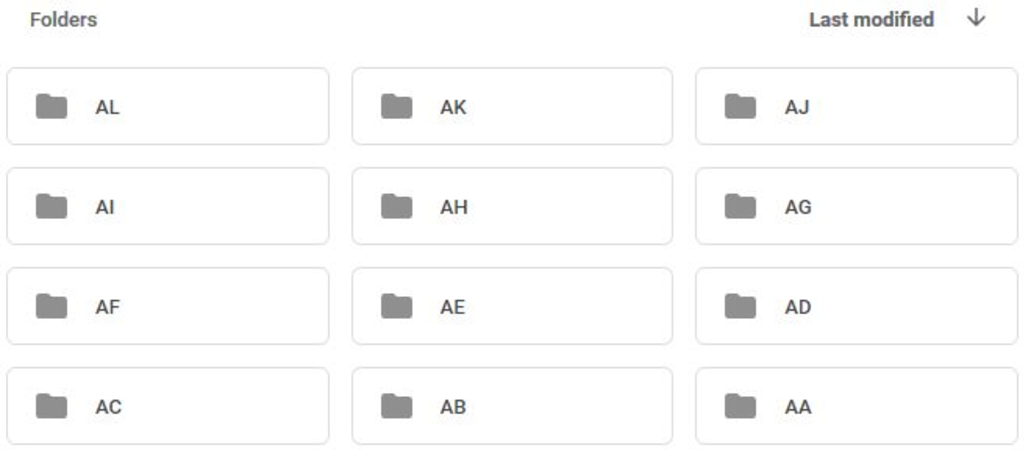
\includegraphics[scale=0.7]{Figures/wikidump.pdf}
\caption{Estructura de datos resultante al extraer un archivo de \textit{Wikipedia}.}
\label{fig:wikidump}
\end{figure}


\textbf{Obtención de datos.} El corpus de Wikipedia fue obtenido del sitio oficial (\url{https://dumps.wikimedia.org/eswiki/}). El corpus obtenido fue del mes de noviembre del año 2018. Estos archivos tienen una estructura específica y la forma recomendada de extraer sus contenidos es utilizando \emph{WikiExtractor} (\url{https://github.com/attardi/wikiextractor}). Esta herramienta permite realizar una extracción que filtra por un parámetro de mínimo de longitud del artículo. Se utilizó este parámetro para filtrar todos los artículos con menos de 10,000 caracteres.

Una vez finaliza la extracción del archivo --- la cual demora una cantidad no despreciable de horas --- se procede a leer y filtrar los documentos. En el caso de este trabajo se ignoraron todos los documentos después de haber acumulado 100 millones de tokens en los textos procesados. Se conservaron 10 millones de tokens adicionales para la validación de resultados.

\begin{table}
\begin{tabular}{| l | l |}

\hline
\textbf{Cadena de caracteres} & \textbf{Resultado tokenizado} \\
\hline
Hola, buenos días. & \texttt{xxbos xxmaj hola , buenos días} \\
HOLA!!! qué bueno verte & \texttt{xxbox xxmaj hola xxrep 3 ! qué bueno verte} \\
Mis audífonos son Sennheiser & \texttt{xxbos xxmaj mis audífonos son xxunk} \\
\hline

\end{tabular}
\caption{Muestras de tokenización utilizando \textit{spaCy} y técnicas de \textit{fastai}}
\label{tab:tokens}
\end{table}

\textbf{Tokenización.} La herramienta utilizada para este proceso fue spaCy (\url{https://spacy.io/}). Esta herramienta tiene soporte para más de 34 idiomas, entre los cuales se incluye el español. Además de esta herramienta se emplean técnicas adicionales como codificar caracteres repetidos o codificar palabras en mayúsculas --- ver tabla \ref{tab:tokens}.

\textbf{Definición de vocabulario.} Unos tokens son codificados como \texttt{xxunk} (token desconocido), esto es debido a la limitación de palabras únicas a codificar. El vocabulario fue limitado a 30,000 tokens únicos.

\begin{figure}
\centering
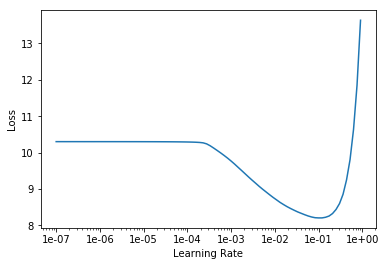
\includegraphics[scale=1]{Figures/lrfinder.png}
\caption{Ilustración de progreso de la función \texttt{lr\_find} de \textit{fast.ai}. Al momento de divergir el método deja de aumentar $\gamma$ y devuelve los resultados.}
\label{fig:lrfind}
\end{figure}

\textbf{Entrenamiento.} Luego tener los datos en el formato adecuado para entrenar el modelo se aplican las técnicas descritas en el capítulo \ref{Chapter3} sobre una red AWD LSTM. Previo a esto se encuentra un $ \gamma $ ideal y eso se hace aprovechando el método \texttt{lr\_find} (figura \ref{fig:lrfind}) de la librería de \emph{fastai} (\url{https://github.com/fastai/fastai}) que emplea el método descrito por \textcite{smith2017convergence}. Se aumenta $\gamma$ a medida que se recorren los ejemplos a entrenar. Si en algún momento diverge el aprendizaje se detiene el método y se imprime la gráfica. Se deberá querer elegir un $\gamma$ que no tenga riesgo de divergir el aprendizaje y que tampoco disminuya la velocidad del proceso. La elección adecuada de este hiper-parámetro en esta etapa es crucial para obtener un modelo en un tiempo razonable, ya que este modelo es el más grande --- en términos de parámetros y datos a procesar --- que requerirá entrenamiento. Vale la pena enfatizar que este proceso se realiza una \emph{única} vez y la definición de modelos clasificadores en un futuro podrá hacer uso del modelo entrenado originalmente.

\subsubsection{Resultados}

Para medir y reportar errores sobre LMs se utiliza la métrica de \textit{perplexity} \parencite{jurafsky2014speech}, la cual es análoga a la entropía. La entropía representa la cantidad de información que se tiene; \textit{perplexity} se puede ver como la cantidad de opciones que se tiene. ¿Qué significa esto? Que mientras menos opciones considere nuestro LM, más estable es y por lo tanto que modela mejor el lenguaje. Se calcula de la siguiente manera:

$$ perplexity = e^{loss} $$

En nuestro caso, se utiliza el valor de pérdida de los datos de validación.

\begin{table}
\centering
\begin{tabular}{|l|l|l|}
\hline
Modelo & Error en validación & \textit{Perplexity} \\
\hline
AWD LSTM & 3.140521 & \textbf{23.1038} \\
QRNN & 3.193912 & 24.2884 \\
\hline
\end{tabular}
\caption{Resultados de los modelos entrenados. La métrica que se utiliza para comparar entre los modelos es \textit{perplexity} la cual indica y representa qué tantas opciones se tienen para la siguiente palabra.}
\label{tab:modresults}
\end{table}

Se entrenaron dos modelos de RNN, uno fue basado directamente de la arquitectura y estrategias de AWD LSTM  y el otro modelo basado en la arquitectura QRNN. Los resultados se muestran en la tabla \ref{tab:modresults}. Sin embargo esta tabla no cuenta la historia completa. El modelo QRNN demoró menos en su entrenamiento de forma no insignificante tomando 13\% menos en entrenarse con resultados muy comparables a los de la red AWD LSTM.

\begin{table}
\centering
\begin{tabular}{|l|l|}
\hline
\textbf{Modelo} & \textbf{\textit{Perplexity}} \\
\hline
Transformer-XL \parencite{dai2019} & \textbf{18.3} \\
\hline
AWD LSTM (propio) & \textbf{23.1038} \\
QRNN (propio) & 24.2884 \\
Activation Mem. \parencite{rae2018} & 29.2 \\
RNN \parencite{goldszmidt2018} & N/A (34\% prec.) \\
RNN \parencite{ingham2018} & 36.1473 \\
\hline

\end{tabular}
\caption{Comparación de LMs con modelos del estado del arte en inglés y modelos de referencia para el español. Menor \textit{perplexity} es mejor. Separamos el modelo \textit{Transformer-XL} ya que utiliza otra arquitectura y está presente en la tabla solamente como referencia al mejor resultado al momento de haber escrito este trabajo.}
\label{tab:lmcomp}
\end{table}

En la tabla \ref{tab:lmcomp} se aprecian distintos LMs los cuales fueron entrenados en distintos datasets. El modelo Transformer-XL \parencite{dai2019} utiliza la nueva tendencia de finales del 2018 y principios de 2019 de usar transformadores en lugar de RNNs, así como propone Google con BERT. El modelo de \textit{Activation Memory} \parencite{rae2018} es un modelo de referencia que utiliza la arquitectura de una RNN simplificando un sub-conjunto de sus parámetros. Los otros dos modelos han sido modelos previamente entrenados con el propósito de ser usados para tareas clasificación en español con ULMFiT. Los datos presentados para los modelos propios fueron el valor de pérdida en un set de validación de 100 millones de tokens elegidos al azar de \textit{Wikiepedia}.

Aunque hay argumentos en contra de usar \textit{perplexity} para comparar LMs de distintos lenguajes o que usan distintos vocabularios \parencite{chen1998evaluation}, se debe tener un marco de referencia. Los modelos con propósitos de usar ULMFiT fueron entrenados de una forma muy similar al propio y son las comparaciones más directas por ser LMs del idioma español.


\subsubsection{Recursos utilizados para entrenamiento}

\textbf{Costo monetario.} Para esta fase de entrenamiento se recurre a los servicios de \textit{Google Cloud} (\href{https://cloud.google.com/free}{https://cloud.google.com}) los cuales son ofrecidos con un beneficio de 300 USD para utilizar durante el primer año. No es necesario ser estudiante o profesor para gozar de este beneficio. Teniendo estos recursos disponibles se optó por utilizar una instance de cómputo \emph{n1-highmem-4} (\url{https://cloud.google.com/compute/docs/machine-types}) la cual cuenta con	el siguiente hardware para el entrenamiento:

%\pagebreak

\begin{itemize}
\item Intel Xeon (Skylake) 4 vCPUs
\item 26 GB de memoria (RAM)
\item nVIDIA V100 GPU -- 16 GB de memoria
\end{itemize}

Lo primordial cuando se trata de entrenamiento de RNNs es la capacidad de cómputo de la GPU. La \textbf{V} en el modelo V100 indica que es de la última generación a la fecha de esta tesis y provee una ventaja significativa comparada con una K80 o P100.

\textbf{Costo de recursos.} El costo total resultante después de entrenar un modelo inicial y funcional llegó a \$ 60.20 USD. Esto fue cubierto por los créditos iniciales ofrecidos por Google. También se debe considerar que este paso se debe realizar \emph{una sola vez} para cada lenguaje. En caso de querer utilizar el modelo entrenado en este trabajo, se podrá hacerlo y se podrá aplicar a otros problemas de clasificación.

\textbf{Costo en tiempo.} Para entrenar los modelos de lenguaje con una estructura AWD LSTM, una época se demora alrededor de una hora. Después de 4 épocas se aproximan los resultados al estado del arte y debe decidirse cuando detener el entrenamiento sin perder la generalidad del sistema.

\subsection{Modelos clasificadores}

\textbf{Procesamiento de datos.} El conjunto de datos principales que se utilizó fue el de PAN17 \parencite{rangel2017overview}. Este conjunto de datos no es típico ya que consta de tuits de un grupo de usuarios. Cada uno de estos tuits --- 100 por usuario --- tiene asociado su usuario el cual tiene las etiquetas de edad y región asignadas. Por lo tanto se puede abordar el problema de distintas formas; se puede tomar cada tuit individual y predecir el género y la región individualmente, sumando después las probabilidades para obtener un veredicto final para el autor o se pueden concatenar los tuits del autor y realizar una solo predicción sobre ese texto completo del autor. Para este trabajo se utilizó cada tuit individual con el fin de poder tener un alcance mayor sobre la tarea de perfilación de autores sobre textos informales.

\begin{table}
\centering
\rowcolors{1}{gray!25}{white}
\begin{tabular}{| p{3cm} | p{9.5cm} |}
\hline
\textbf{Estado del texto} & \textbf{Resultado} \\
\hline
Original & \texttt{\#igualdaddegenero y \#mediosdecomunicacion http://t.me/ssbM} \\
Sin normalizar & \texttt{xxunk xxunk y xxunk xxunk xxunk} \\
Normalizado & \texttt{xxhashtag igualdad enero y xxhashtag medios comunica xxurl} \\
\hline
\end{tabular}
\caption{Ejemplificación de normalización de textos informales obtenidos del dataset PAN17 para la tarea de perfilación de autores. El proceso de normalización permite extraer información de los \textit{tokens} que son menciones de usuario y \textit{hashtags}. En la tabla se aprecia un ejemplo real con drásticos cambios dependiendo de procesamiento.}
\label{tab:pan17preproc}
\end{table}

\textbf{Pre-procesamiento y tokenización.} El procesamiento constó de normalizar los \textit{tokens} especiales de los textos (ver tabla \ref{tab:pan17preproc}); en particular se normalizaron las menciones de usuario y los \textit{hashtags}. Este proceso consistió en ordenar los \textit{tokens} del vocabulario del modelo pre-entrenado de \textit{Wikipedia} y buscar las instancias encontradas en los \textit{tokens} de interés. Luego de haber hecho esto, anteponer un \textit{token} especial que indique que se encontraba ahí originalmente, por ejemplo \texttt{xxhashtag}. Se tokenizan los datos de la misma manera en que se tokenizaron los datos en la fase de modelo de lenguaje; utilizando \textit{spaCy}.

\textbf{Afinación de LM.} Después de haber entrenado el modelo de lenguaje se procede a una fase de afinación \parencite{howard2018}. Se emplean las técnicas descritas en el capítulo \ref{Chapter3} para poder afinar el modelo. Este proceso se realiza con los datos de la tarea en específico. Se adapta el formato de los datos de clasificación a datos para entrenamiento de un LM y se afina el modelo para textos de este dominio específico. Sobre la métrica de \textit{perplexity} o la precisión no se pone mayor énfasis, lo importante será que la estructura general de los textos y el vocabulario que se use refleje los datos reales del problema específico.

\begin{comment}
resultados en afinamiento de lm aca. grafica? tabla?
\end{comment}

\textbf{Entrenamiento de los modelos clasificadores.} Al tener el LM afinado se procede a entrenar un clasificador. Este proceso es descrito en la sección \ref{sec:nlpprocess}. A continuación se detallan las decisiones tomadas.

\begin{figure}
\centering
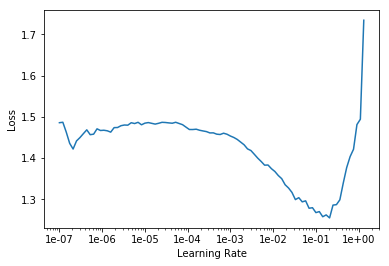
\includegraphics[scale=1]{Figures/clas_lrfinder.png}
\caption{Evolución de la pérdida conforme se cambia la tasa de aprendizaje en el clasificador. Al igual que con el LM, se deberá elegir un valor óptimo para mayor eficiencia.}
\label{fig:claslr}
\end{figure}

\textbf{Entrenamiento del clasificador.} Antes de comenzar con el entrenamiento se deben elegir los hiper-parámetros adecuados. Primero se eligió un peso para los parámetros de \textit{dropout} (basado en pruebas empíricas) y después se eligió un $\gamma$ óptimo basado en la herramienta de \texttt{lr\_find} (figura \ref{fig:claslr}). Los valores elegidos fueron \texttt{dropout = 0.3} y un $\gamma$ inicial con valor de \texttt{1e-2}. Se habla de un $\gamma$ inicial ya que en el entrenamiento del modelo clasificador se aplica el concepto de usar un $\gamma$ cíclico \parencite{smith2017convergence} abordado en el capítulo \ref{Chapter3}.

\begin{figure}
\centering
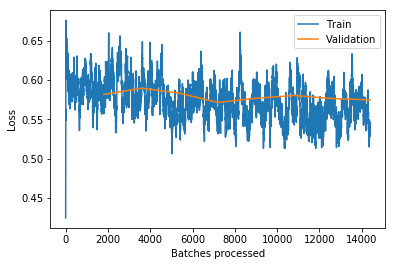
\includegraphics[scale=1]{Figures/clas_epochs.png}
\caption{Avance de pérdida conforme avanzan las épocas de entrenamiento. Menor es mejor.}
\label{fig:clasepochs}
\end{figure}

El entrenamiento de un clasificador con pocos datos no deberá tomar mucho tiempo y los resultados deberán ser satisfactorios aplicando los temas expuestos en este trabajo. En la figura \ref{fig:clasepochs} se puede apreciar como la evolución de pérdida avanza lentamente a través de las épocas y converge en un valor después de un número de épocas relativamente bajo. Sin embargo, es posible continuar con el entrenamiento hasta lidiar con \textit{overfitting}. Este problema surge cuando se han afinado tanto los parámetros del modelo que el proceso de \textit{backpropagation} empieza a ajustarse conforme solamente los datos de entrenamiento y no el problema en sí. La manera más fácil de detectar este fenómeno es con la comparación de resultados sobre la función de pérdida de los datos de entrenamiento con los datos de evaluación. Si el valor de pérdida para ambos conjuntos de datos disminuye significa que el entrenamiento se está realizando con éxito. Si en algún momento el valor de pérdida para los datos de entrenamiento continua disminuyendo pero al mismo tiempo el valor de pérdida para los datos de validación aumenta significa que ya no estamos obteniendo resultados que puedan ser generalizados a datos no antes vistos.

\begin{comment}
grafica de overfitting
\end{comment}



\section{Resultados}

Se ha dicho que para RNNs y técnicas de aprendizaje profundo no han tenido el mismo éxito que en otras tareas debido a la dificultad que un modelo de aprendizaje profundo tiene al aprender la cantidad de parámetros inmensa con pocos datos \parencite{zampieri2017, malmasi2016discriminating}. Esta tarea es por lo tanto ideal para poder determinar la capacidad real la transferencia de aprendizaje en NLP y sobre todo cuando las instancias de aprendizaje son limitadas.

Los datos y resultados en referencia a predicción de región y género provienen del reporte de la competencia PAN17 \parencite{rangel2017overview} y proveen un contexto para la tarea del trazo de perfiles de autores. Debido a que los conjuntos de datos de pruebas son los mismos, las comparaciones se podrán hacer de forma directa. Se realiza una comparación con datos exclusivamente del idioma español. Los modelos a comparar son los siguientes:

\begin{itemize}
\item TF-IDF + CNN \parencite{schaetti2017author}
\item RNN \parencite{kodiyan2017author}
\item AVG DNN \parencite{franco2017author}
\item CNN + RNN + Attention \parencite{miura2017author}
\end{itemize}

Para estos resultados se utiliza la métrica usada en la competencia PAN17 la cuál es:

% \: es un espacio de mediana distancia

$$ Acc_{cat} = \frac{Predicciones\: correctas}{Total\: de\: predicciones} $$

Donde $cat$ es la categoría sobre la cual se está prediciendo. Las predicciones son aplicadas sobre los datos de validación, los cuales fueron segmentados por el equipo organizador de PAN17 los cuales cuenta con 2,800 autores, cada uno asociado a 100 tuits.

\subsection{Predicción de género}

La predicción de género sobre un texto anónimo se realizó basado en datos de tuits. La clasificación se llevó a cabo en dos niveles. Se realizó una predicción a nivel de tuit individual y una predicción a nivel de autor.

\begin{table}
\centering
\begin{tabular}{r | c c}
\multicolumn{3}{c}{\textbf{Referencia}} \\
\textbf{Predicción} & Femenino & Masculino \\
\hline
Femenino & 83110 & 49573 \\
Masculino & 56890 & 90427 \\
\end{tabular}
\caption{Matriz de confusión de resultados sobre predicción de género en tuits individuales.}
\label{tab:gender_indvtweet}
\end{table}

En la tabla \ref{tab:gender_indvtweet} se aprecian los resultados de las predicciones sobre tuits individuales. La evaluación de la métrica con estos datos sería entonces:

$$ Acc_{gender\_idv} = \frac{173,537}{280,000} = 0\text{.}6198 $$

\begin{table}
\centering
\begin{tabular}{r| c c}
\multicolumn{3}{c}{\textbf{Referencia}} \\
\textbf{Predicción} & Femenino & Masculino \\
\hline
Femenino & 963 & 283 \\
Masculino & 437 & 1117 \\
\end{tabular}
\caption{Matriz de confusión de resultados de predicciones por autor.}
\label{tab:gender_authtweet}
\end{table}

La predicción sobre los autores es basada en las predicciones sobre tuits individuales. Esto resulta en una suma ponderada de las predicciones individuales descrita como
\[ \phantom{,}\hat{p}_a (\mathbf{X}) = \max \sum_{n = 1}^{100} p(X_n), \]
donde $\mathbf{X}$ representa una matriz de probabilidades; las filas representan tuits individuales y las columnas las probabilidades de que el tuit pertenezca a la categoría de esa columna (p.e. el género femenino).

Dada la anterior tenemos la tabla \ref{tab:gender_authtweet} y un resultado de
\[ \phantom{.}Acc_{gender} = 0\text{.}7429. \]

La sumatoria ponderada resulta en un sistema similar a un ensamble de modelos los cuales toman prioridad según la confianza que tengan en su predicción. Debido a esto, el resultado aumenta en la métrica considerablemente.

\begin{table}
\centering
\rowcolors{2}{gray!25}{white}
\begin{tabular}{p{9.5cm} p{3cm}}
\textbf{Modelo} & \textbf{Resultado} \\
\hline
TF-IDF + CNN \tblshort\parencite{schaetti2017author} & 0.7150 \\
RNN \tblshort\parencite{kodiyan2017author} & 0.7217 \\
RNN + Transfer Learning (propio) & 0.7429 \\
AVG DNN \tblshort\parencite{franco2017author} & \textbf{0.7721} \\
\hdashline
\rowcolor{white}
CNN + RNN + Attention \tblshort\parencite{miura2017author} & \textbf{0.8118} \\

\end{tabular}
\caption{Comparación de modelos de aprendizaje profundo en la tarea de predicción de género --- mayor es mejor. El modelo de \tblshort\textcite{miura2017author} se separa ya que es un ensamble de modelos y no se puede hacer una comparación directa.}
\label{tab:pan17gender}
\end{table}

Al comparar el modelo propio con los modelos de aprendizaje profundo presentados en la competencia PAN17 (tabla \ref{tab:pan17gender}) se puede apreciar que los resultados obtenidos son del estado del arte para RNN, siendo solamente superado por un AVG DNN y un ensamble de CNN, RNN y elementos de atención.

\subsection{Predicción de región}

La predicción de género sobre un texto anónimo se realizó basado en datos de tuits. La clasificación se llevó a cabo en dos niveles. Se realizó una predicción a nivel de tuit individual y una predicción a nivel de autor.

\begin{table}
\centering
\begin{tabular}{r | c c c c c c c}
\multicolumn{3}{c}{\textbf{Referencia}} \\
\textbf{Predicción} & AR & CL & CO & MX & PE & ES & VZ\\
\hline
AR & 22,610 & 3,013 & 3,147 & 2,220 & 3,783 & 2,558 & 2,188 \\
CL & 3,064 & 21,058 & 2,988 & 3,034 & 3,760 & 2,599 & 2,454 \\
CO & 3,435 & 2,993 & 20,007 & 4,401 & 4,251 & 2,746 & 3,696 \\
MX & 2,554 & 3,429 & 3,977 & 18,803 & 4,173 & 3,681 & 3,616 \\
PE & 2,992 & 3,780 & 3,544 & 3,542 & 17,812 & 2,552 & 2,605 \\
ES & 3,331 & 3,565 & 3,519 & 5,131 & 3,662 & 23,722 & 3,689 \\
VZ & 2,014 & 2,162 & 2,818 & 2,869 & 2,559 & 2,142 & 21,752 \\
\end{tabular}
\caption{Matriz de confusión de resultados sobre predicción de región en tuits individuales.}
\label{tab:region_indvtweet}
\end{table}

De la misma manera que con las predicciones de género, en la tabla \ref{tab:region_indvtweet} se aprecian los resultados de las predicciones sobre tuits individuales. La evaluación de la métrica con estos datos --- siendo esta solo indicativa --- sería entonces la siguiente:

$$ Acc_{region\_idv} = \frac{145,764}{280,000} = 0\text{.}5206 $$

\begin{table}
\centering
\begin{tabular}{r| c c c c c c c}
\multicolumn{3}{c}{\textbf{Referencia}} \\
\textbf{Predicción} & AR & CL & CO & MX & PE & ES & VZ\\
\hline
AR & 381 & 5 & 7 & 5 & 14 & 1 & 7 \\
CL & 2 & 370 & 2 & 3 & 4 & 1 & 1 \\
CO & 2 & 3 & 367 & 10 & 9 & 3 & 8 \\
MX & 3 & 5 & 4 & 364 & 9 & 3 & 9 \\
PE & 4 & 7 & 8 & 3 & 353 & 3 & 4 \\
ES & 5 & 5 & 8 & 13 & 4 & 388 & 17 \\
VZ & 3 & 5 & 3 & 2 & 7 & 1 & 354 \\
\end{tabular}
\caption{Matriz de confusión de resultados de predicción de región por autor.}
\label{tab:region_authtweet}
\end{table}

La predicción sobre los autores basada en la suma ponderada tenemos la tabla \ref{tab:region_authtweet} y un resultado de
\[ \phantom{.}Acc_{region} = 0\text{.}9207. \]

La sumatoria ponderada resulta en un resultado mucho mayor que el de las predicciones individuales. Esto puede deberse a dos cosas:

\begin{itemize}
\item Muchos tuits son muy limitados en su número de caracteres por lo que algunos no revelarán mucha información acerca del autor por sí solos.
\item La cobertura de vocabulario con palabras regionales disminuye por lo que algunos tuits individuales con palabras claves no proveen mucha información.
\end{itemize}

\begin{table}
\centering
\rowcolors{2}{gray!25}{white}
\begin{tabular}{p{9.5cm} p{3cm}}
\textbf{Modelo} & \textbf{Resultado} \\
\hline
TF-IDF + CNN \tblshort\parencite{schaetti2017author} & \textbf{0.9336} \\
RNN \tblshort\parencite{kodiyan2017author} & 0.9143 \\
RNN + Transfer Learning (propio) & 0.9207 \\
AVG DNN \tblshort\parencite{franco2017author} & 0.9000 \\
\hdashline
\rowcolor{white}
CNN + RNN(Att.) \tblshort\parencite{miura2017author} & \textbf{0.9271} \\

\end{tabular}
\caption{Comparación de modelos de aprendizaje profundo en la tarea de predicción de región --- mayor es mejor. El modelo de \tblshort\textcite{miura2017author} se separa ya que es un ensamble de modelos y no es posible hacer una comparación directa.}
\label{tab:pan17region}
\end{table}

Nuevamente se comparan los resultados con los modelos de aprendizaje profundo de PAN17 (tabla \ref{tab:pan17region}). Una combinación de TF-IDF y CNN \parencite{schaetti2017author} logró clasificar de la mejor manera; el modelo propio obtiene la segunda mejor precisión en modelos simples y la tercera considerando el ensamble de modelos CNN y RNN de \textcite{miura2017author}.



